\section{Method}
\label{sec:model}

\begin{figure*}[t]
\centering
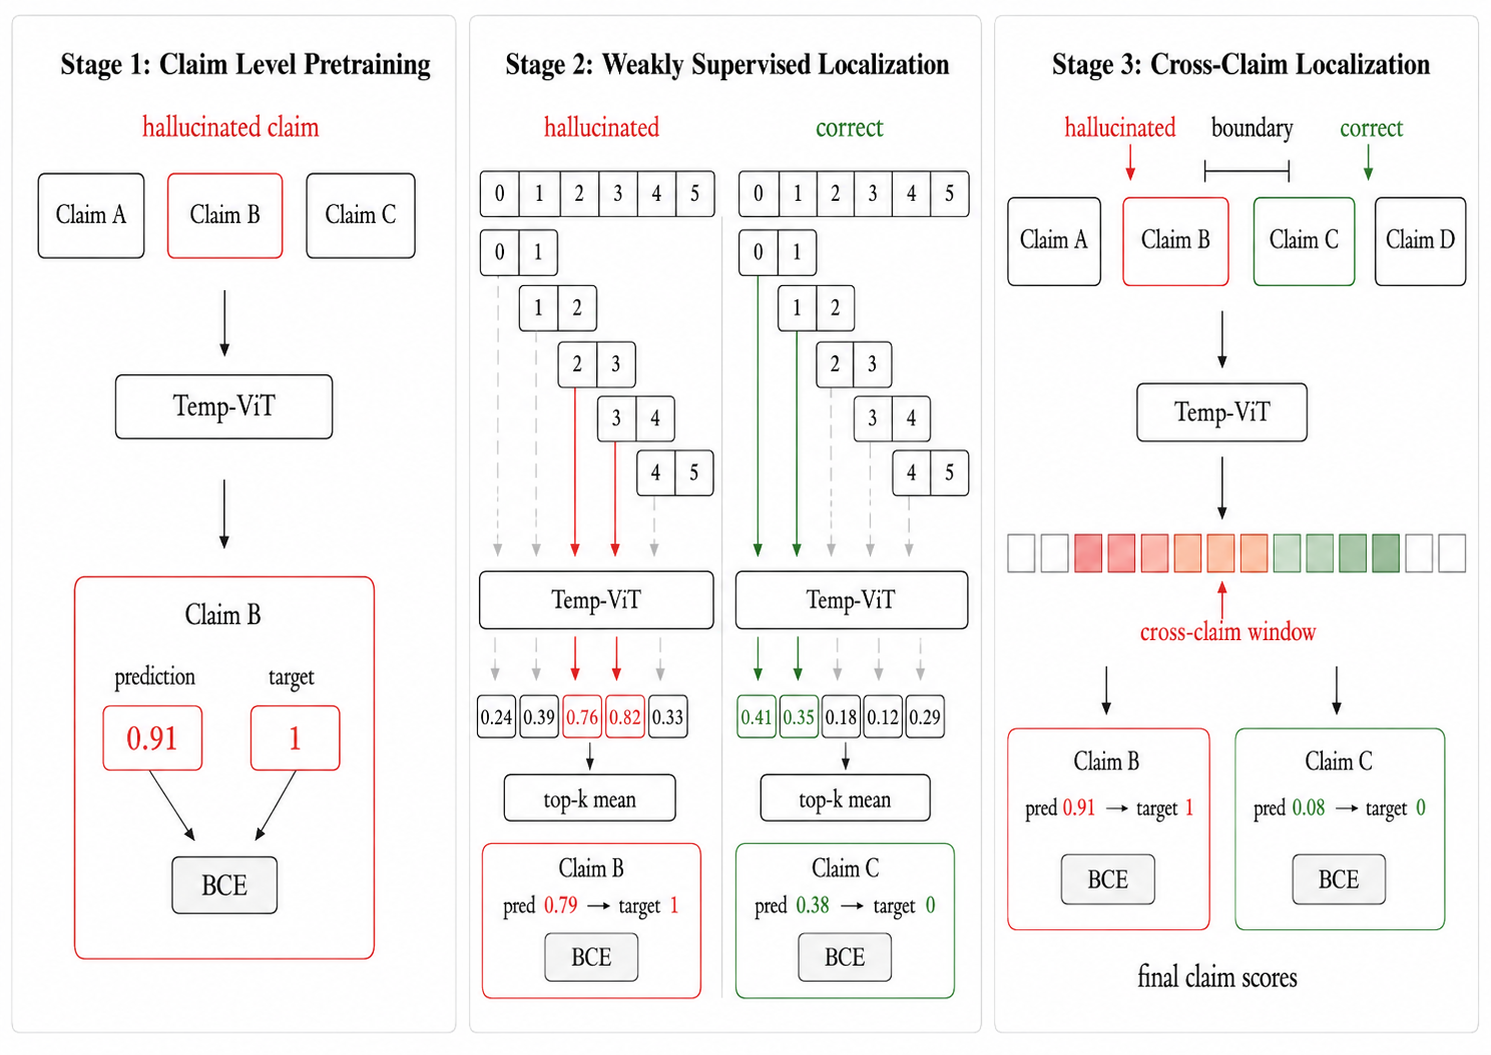
\includegraphics[width=0.95\linewidth]{figs/fig1_overview.png}
\caption{Three-stage Temp-ViT.
\textbf{Stage~1} (top): an ACT-ViT encoder maps a per-atom activation
tensor $A \in \mathbb{R}^{L \times T \times D}$ to an atom-level
uncertainty score via Pool $\to$ per-LLM linear adapter $\to$ ViT
$\to$ linear head.
\textbf{Stage~2} (middle): the encoder is frozen and applied to
centered length-$W$ token windows; a Mamba-2 temporal head emits one
logit per window, aggregated by top-$k$ MIL into an atom-level score.
\textbf{Stage~3} (bottom): the head is fine-tuned on whole passages
with noisy per-atom labels $\tilde{y}_m$ from atomic-fact
verification; per-token logits are smoothed and aggregated within
each atom span $(\ell_m, r_m)$ via a per-atom BCE, so the head ranks
uncertainty across atoms rather than scoring each in isolation.}
\label{fig:overview}
\end{figure*}


Figure~\ref{fig:overview} illustrates TPE's three-stage pipeline over
hidden-state activations $A \in \mathbb{R}^{L \times T \times D}$.
Stage~1 trains a sequence encoder $E_\theta$ on isolated labeled
segments, mapping $A$ to an embedding $e$ and sequence logit $z$.
Stage~2 slices the same activation tensor into centered length-$W$
windows $A^{(1)},\ldots,A^{(T)}$, adds a Mamba-2 temporal head
\citep{albertgu2024}, and trains per-window logits
$\hat{z}^{(1)},\ldots,\hat{z}^{(T)}$ through a top-$k$ MIL sequence
loss. Stage~3 freezes $E_\theta$ and refines the temporal head on
whole passages using claim spans $(\ell_m,r_m)$ and auxiliary labels
$\tilde{y}_m$, so the same token-window scores can be aggregated to
sentence, claim, and sequence predictions.

\subsection{Problem setup and notation}
\label{sec:notation}

Given an LLM $M$ and a generated response of length $T$, we collect
hidden-state activations $A \in \mathbb{R}^{L \times T \times D}$
over $L$ layers and hidden dimension $D$. For localization, TPE also
uses the windowed view
$A^{(t)} \in \mathbb{R}^{L \times W \times D}$, a length-$W$ slice
centered at generated position $t$. Training examples provide a
sequence label $y \in \{0,1\}$, and long-form corpora additionally
provide noisy claim labels
$\{(\ell_m, r_m, \tilde{y}_m)\}_{m=1}^{M}$ from claim-level
verification. The model predicts a sequence uncertainty score
$\hat{p}$ and per-window scores
$\{\hat{p}^{(t)}\}_{t=1}^{T}$; extended notation, dataset
construction, white-box assumptions, and off-domain generalization
are deferred to Appendix~\ref{app:extended}.

\subsection{Stage 1: Encoder}
\label{sec:act_vit_subsec}

The encoder has three components. Pool applies adaptive
max-pooling over $(L, T)$ to a target spatial size $(L_p, T_p)$,
yielding $A_p \in \mathbb{R}^{L_p \times T_p \times D}$. LA
is a per-LLM linear adapter
$LA_M : \mathbb{R}^D \to \mathbb{R}^{D'}$ that aligns hidden
dimensions across models, motivated by recent evidence that LLM
representations can be put in
approximate correspondence by linear maps
\citep{huh2024,moschella2022,kornblith2019}. The Perception Encoder
processes the pooled $(L_p \times T_p)$ activation image as a visual
input and returns a dense embedding for the layer-token plane
\citep{bolya2025perceptionencoder}. A linear head emits the Stage-1
logit $z$, trained with
$\mathcal{L}_{1} = \mathrm{BCE}(\sigma(z), y)$ where $y$ is the
sequence label; the pre-head features form the embedding reused by
Stages 2 and 3.

\subsection{Stage 2: Temporal Localization with Top-$k$ MIL}
\label{sec:temporal_head}

For each generated position $t$, we extract the windowed activations
$A^{(t)} \in \mathbb{R}^{L \times W \times D}$ as $W$ token
columns of $A$ centered at $t$. The same Pool is reused with a
smaller token target $(L_p, W_p)$, and $E_\theta$ produces a
per-window embedding $e^{(t)} \in \mathbb{R}^{d}$. Stacking the $T$
windows yields $E \in \mathbb{R}^{T \times d}$. A residual stack of
Mamba-2 blocks processes $E$ along the token axis followed by a
linear head:
$\hat{z}^{(t)} = h(\mathrm{Mamba\text{-}2}(E)_t)$.
Mamba-2's linear-time selective state-space recurrence makes Stage 2
viable for real-time streaming, where each new token requires only a
constant-memory update.

Because only sequence-level labels are
available, we train via top-$k$ MIL: after masking padded positions,
take the $k$ largest per-window logits and average them into one
sequence-level logit:
\begin{equation}
\hat{z} = \tfrac{1}{k}\!\!\!\sum_{t \in \mathrm{Top}_k(\{\hat{z}^{(t)}\}_t)}\!\!\!\hat{z}^{(t)}, \qquad \hat{p} = \sigma(\hat{z}),
\end{equation}
and supervise with $\mathcal{L}_{2} = \mathrm{BCE}(\hat{p}, y)$.
Mean-of-top-$k$ avoids the outlier sensitivity of max and the signal
dilution of a full mean while keeping the supervision sequence-level.

\subsection{Stage 3: Cross-Claim Refinement}
\label{sec:stage3}

Stages 1 and 2 see one claim segment at a time and do not observe
how the uncertainty activation signal changes across neighboring
claims. Mixed-content windows, whose receptive field straddles
hallucinated and supported tokens, combine signal regimes that
single-claim training cannot disentangle. Stage 3 therefore freezes
$E_\theta$ and fine-tunes the temporal head on whole passages with
claim spans $\{(\ell_m, r_m)\}_{m=1}^{M}$ and noisy labels
$\tilde{y}_m$. The Stage-2 detector emits passage-level per-token
logits, which are locally smoothed and aggregated within each claim
by a top-$k$ mean to form $\hat{z}_m$. A per-claim BCE loss
$\mathcal{L}_{3}$ trains the head to model the signal profile within
and across claims rather than scoring each claim in isolation; the
exact smoothing and claim aggregation are given in
Appendix~\ref{app:extended}.

At inference time, a single forward through the Stage-3 detector
yields the per-token logits over the whole passage, from which we
read off (i) the per-token / per-window scores
$\{\sigma(\hat{z}^{(t)})\}_{t=1}^{T}$ for token-level localization;
(ii) per-sentence scores obtained by aggregating the smoothed
per-token logits within each sentence span with the same top-$k$
mean; (iii) per-claim scores $\{\sigma(\hat{z}_m)\}_m$ when claims
are available; and (iv) a sequence-level score by reusing the
Stage-2 top-$k$ MIL aggregation.
